\section*{Problem 6:}
We used our implementation of Lanczos-based approach and run it on the data of \texttt{FP\_Ex2.mat}. Figure~\ref{fig:fig2} shows the results with $s0 = 10^{10}$ and $k = 1000$.  Function \texttt{Figure\_2()} in \texttt{driver.m} file generates this plot. 

\begin{figure}[!tbh]
\centering        
   \subfloat {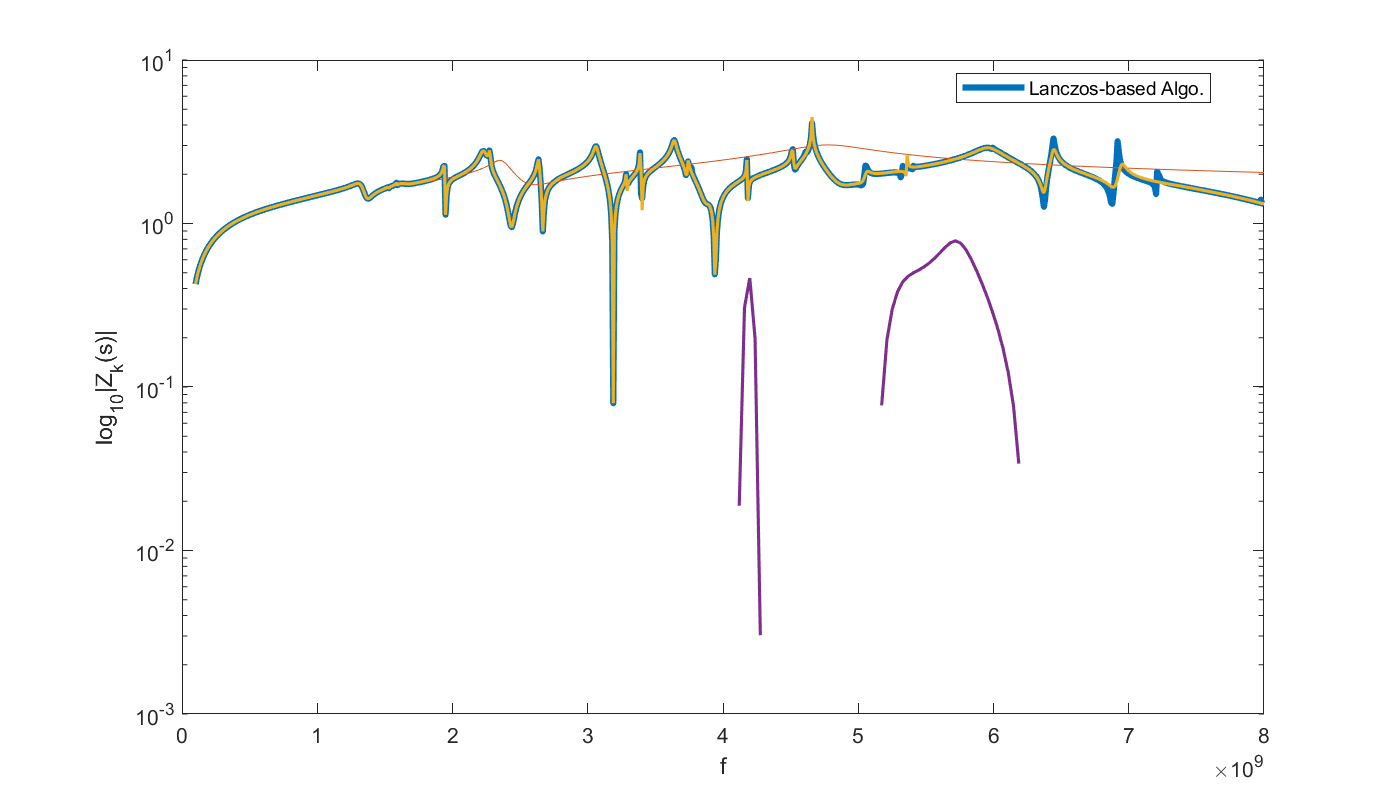
\includegraphics[width=0.85\textwidth]{../code/figure2.png}}
   \caption{Results of the Lanczos-based approach on Example 2 input with $s0 = 10^{10}$ and $k = 1000$ }
   \label{fig:fig2}
\end{figure}




\begin{table}[!tbh]
 \centering    
\begin{tabular}{ |p{3.0cm}|p{1.5cm}| p{4cm}||}
\hline
 $s_{0}$  & $k$ & Time           \\ \hhline{|=|=|=|}   
 $10^{10} + 2 \pi i f_{avg}$ & &  \\
 $10^{10} + 2 \pi i f_{min}$ & &  \\
 $10^{10} + 2 \pi i f_{max}$ & &  \\
 $10^{?} $                   & &  \\
 $10^{10}$                   & &  \\  
\hline
\end{tabular} 
\caption{Experimenting with Lanczos approach using different $s_{0}$ values ($f_{avg} = \frac{f_{min}+f_{max}}{2}$) }
   \label{tab:s02}
\end{table}